\chapter{Colour Spaces and Systems}
\label{s:spaces}

The colour information used in this book is reported in a wide
variety of colour spaces. The main colour space used in my own
experiments is CIE 1967 $L^*a^*b^*$, but data reported in incorporated
studies are often reported in other colour systems. Some studies
\citep[e.g.][]{lillo07locating} used the CIE 1967 $L^*u^*v^*$ colour
space whereas others \citep[e.g.][]{sturges95location} used the
Munsell colour system to report their results. The vision system of
the Sony humanoid robots uses the YCbCr colour model to encode the
colour information of the objects they perceive.

This chapter introduces the different colour spaces and systems and
the functions that are used to convert this data from one colour
system into another, as shown in Figure \ref{f:conversions}. Some
conversions are impossible to compute in one step and hence require
some intermediary steps. Most of these functions are based on Bruce
Lindblooms's website\footnote{http://www.brucelindbloom.com}.

\begin{figure}[htb]
\begin{center}
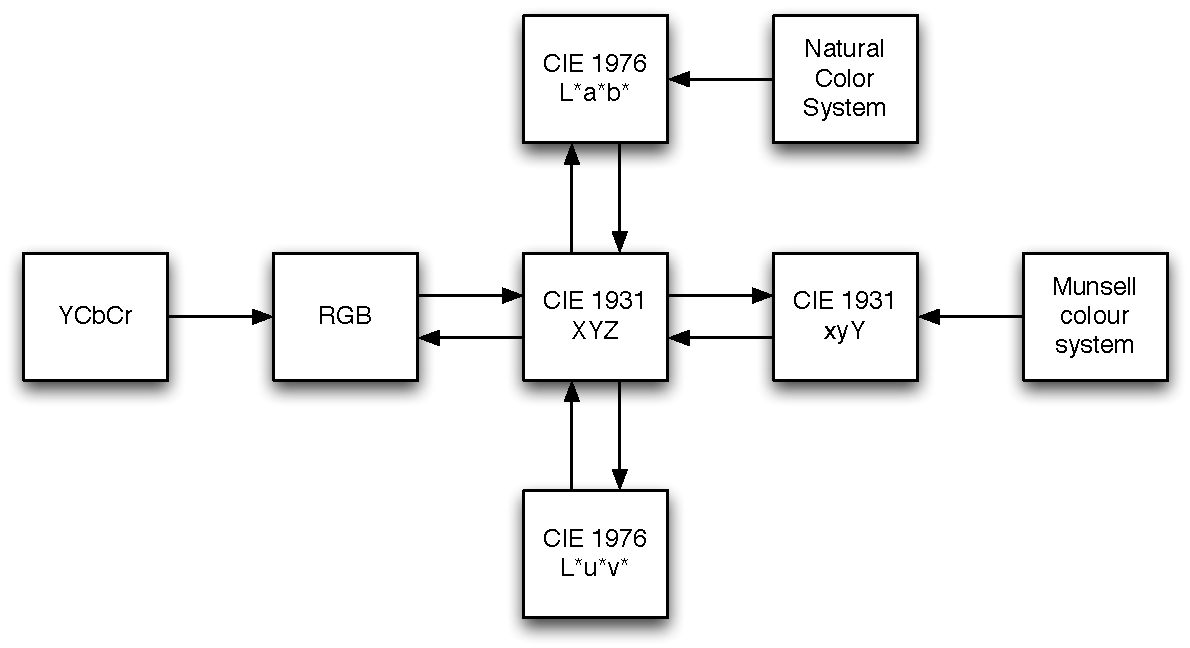
\includegraphics[width=\textwidth]{./spaces/figures/conversions.pdf}
\caption[Conversion diagram between different colour models and
spaces]{A diagram representing the conversions between the different
  colour models and spaces. To convert colour information from the
  YCbCr colour model to the CIE 1967 $L^*a^*b^*$ colour space for
  example, it first needs to be converted to RGB which can be
  converted to CIE 1931 XYZ which can finally be converted to CIE 1967
  $L^*a^*b^*$.}
\label{f:conversions}
\end{center}
\end{figure}

\section{CIE 1931 XYZ colour space}
\label{s:xyz}
\is{colour space!CIE 1931 XYZ}
\is{CIE 1931 XYZ|see{colour space}}

Central to the conversion diagram (Figure \ref{f:conversions}) is the
XYZ colour space. The XYZ colour space was established by the
\emph{Commission Internationale de l'Eclairage} (CIE) in 1931. It standardised
the colour-matching functions which describe how to combine the
different amounts of primaries into unique colours and how to establish
the primaries themselves. It was based on two experiments
\citep{wright28, guild31} which independently estimated the
colour-matching functions for humans with normal colour vision, based
on the principles of trichromacy and Grassmann's laws of additive
colour mixture. The experiments matched to such a level of degree that
the CIE decided to put them forward as the standard set of
colour-matching functions.

Although the XYZ primaries are based on studies of human subjects,
they are imaginary and do not map directly on the primaries
established by the studies. This is mainly done to eliminate some
mathematical properties of the original colour-matching functions and
to incorporate the results into the previously established system of
photometry. More exactly, the primaries for X and Z are imaginary as
they do not produce any luminance response, whereas the primary for Y
is the luminance response \citep{fairchild98color}.

\subsection{Illuminants and chromatic adaptation}

As the appearances of colours change under different light sources,
these sources are also incorporated in the model as idealised
illuminants which reflect their spectral power distribution. These
distributions determine how much each wavelength contributes to the
total illumination. Some of them, such as illuminant A, try to model a
typical domestic lighting, whereas others, such as illuminants C and
D65, try to reconstruct natural daylight conditions. In all reported
experiments, D65 is used as standard illuminant. For each illuminant a
reference white can be defined which represents the colour `white'
under such illuminant. The reference whites for some illuminants are
shown in Table \ref{t:reference-whites}.

\begin{table}
\begin{center}
\begin{tabular}{|c|c|c|c|}
\hline
Illuminant & X & Y & Z \\
\hline
A & 1.09850 & 1.00000 & 0.35585 \\
C & 0.98074 & 1.00000 & 1.18232 \\
D65 & 0.95047 & 1.00000 & 1.08883 \\
\hline
\end{tabular}
\end{center}
\caption{Reference white tristimulus values for illuminants A, C and D65}
\label{t:reference-whites}
\end{table}

To adapt $XYZ$ values from one illuminant to another, several
chromatic adaptation algorithms have been proposed. All these
algorithms first transform the $XYZ$ values into the cone response
domain before scaling the actual values depending on the source and
target illuminant. The algorithms differ in how they do the
transformation to the cone response domain. The Bradford method is
considered to be the best one.

All steps of this transformation can be compiled into one matrix
multiplication. To convert from illuminant C to illuminant D65,
Equation \ref{e:c-to-d65} was used\footnote{More chromatic
  transformations can be found on Bruce Lindbloom's website:\\
  \url{http://www.brucelindbloom.com/Eqn_ChromAdapt.html}.}.

\begin{equation}
\begin{bmatrix}
  X_{D65} \\ Y_{D65} \\ Z_{D65}
\end{bmatrix}
=
\begin{bmatrix}
 0.9904476 & -0.0071683 & -0.0116156 \\
-0.0123712 & 1.0155950 & -0.0029282 \\
-0.0035635  & 0.0067697 & 0.9181569
\end{bmatrix}
\begin{bmatrix}
  X_{C} \\ Y_{C} \\ Z_{C}
\end{bmatrix}
\label{e:c-to-d65}
\end{equation}

\subsection{Chromaticity diagrams and CIE xyY colour space}
\is{colour space!CIE xyY}
\is{CIE xyY|see{colour space}}

Chromaticity diagrams were developed to provide a convenient
two-dimensional representation of colour which removes the luminance
information. This is achieved by means of a one-point perspective
projection onto the unit plane of the XYZ colour space. The
transformation from the $XYZ$ coordinates to the $xy$ plane can be
computed using Equations in \ref{e:xyz-to-xyy}.

\begin{equation}
x = \frac{X}{X + Y + Z} \qquad
y = \frac{Y}{X + Y + Z} \qquad
z = \frac{Z}{X + Y + Z}
\label{e:xyz-to-xyy}
\end{equation}

Given the nature of the projection the third chromaticity coordinate
$z$ can always be computed from the other two because the three sum
to unity. $z$ can also be computed using Equation \ref{e:xy-to-z}.

\begin{equation}
z = 1.0 - x - y
\label{e:xy-to-z}
\end{equation}

The inverse transformation from chromaticy coordinates $x$ and $y$ can
only be computed when one of the original tristimulus values is
given. In most cases this is the luminance value $Y$. The inverse
transformation from xyY to XYZ is computed using Equations
\ref{e:xyy-to-xyz}

\begin{equation}
X = \frac{xY}{y} \qquad
Z = \frac{zY}{y} =  \frac{(1.0-x-y)Y}{y}
\label{e:xyy-to-xyz}
\end{equation}

\section{CIE 1976 L*a*b*}
\label{s:lab}
\is{colour space!CIE 1976 \emph{L*a*b*}}
\is{CIE 1976 \emph{L*a*b*}|see{colour space}}


The CIE 1976 \emph{L*u*v*} and \emph{L*a*b*} (CIELUV and CIELAB for
short) colour spaces were designed to provide uniform practices for
the measurement of colour differences. To determine the colour
difference ($\Delta E^*_{ab}$ or $\Delta E^*_{uv}$) it suffices to use
the Euclidean distances between two colours represented in these
spaces. To achieve this goal, the colour spaces are extended with
dimensions that correlate to lightness, chroma and hue. These spaces
also incorporate features to account for chromatic adaptation and
nonlinear visual responses.

In the CIELAB space, the \emph{L*} dimension represents lightness, the
\emph{a*} dimension approximately redness-greenness and the \emph{b*}
dimension approximately yellowness-blueness. Chroma ($C^*_{ab}$) and
hue ($h_{ab}$) can be computed by the Equations in
\ref{e:lab-chroma-hue}. The value for \emph{L*} ranges from 0 (black)
to 100 (white). The values for \emph{a*} and \emph{b*} can be both
positive and negative and are only limited by the physical properties
of materials.  $h_{ab}$ is expressed as an angle in degrees. The
\emph{L*}, $C^*_{ab}$ and $h_{ab}$ form a cylindrical representation
of the same space.

\begin{equation}
C^*_{ab} = \sqrt{\left(a^{*^2} + b^{*^2} \right)} \qquad h_{ab} = \tan^{-1} \frac{b^*}{a^*}
\label{e:lab-chroma-hue}
\end{equation}

\subsection{Conversion}

The equations to convert CIE 1931 XYZ coordinates to CIE 1976
\emph{L*a*b*} coordinates are shown in Equations
\ref{e:xyz-to-lab-first}-\ref{e:xyz-to-lab-last}, where $\epsilon$ and
$\kappa$ have identical values as defined in Equations \ref{e:epsilon}
and \ref{e:kappa}. This conversion requires a reference white
$\begin{bmatrix}X_r & Y_r & Z_r\end{bmatrix}$ which for my experiments
is chosen based on illuminant D65 (see Table
\ref{t:reference-whites}).

\begin{align}
L^{*}& = 116f_y - 16
\label{e:xyz-to-lab-first} \\
a^{*}& = 500(f_x - f_y) \\
b^{*}& = 200(f_x - f_y) \\
f_x& = \left\{
\begin{aligned}
&\sqrt[\leftroot{-1}\uproot{2}3]{x_r} & \quad x_r > \epsilon \\
&\frac{\kappa x_r + 16}{116} & \quad x_r \leq \epsilon
\end{aligned}
\right. \\
f_y& = \left\{
\begin{aligned}
&\sqrt[\leftroot{-1}\uproot{2}3]{y_r} & \quad y_r > \epsilon \\
&\frac{\kappa y_r + 16}{116} & \quad y_r \leq \epsilon
\end{aligned}
\right. \\
f_z& = \left\{
\begin{aligned}
&\sqrt[\leftroot{-1}\uproot{2}3]{z_r} & \quad z_r > \epsilon \\
&\frac{\kappa z_r + 16}{116} & \quad z_r \leq \epsilon
\end{aligned}
\right. \\
x_r& = \frac{X}{X_r} \\
y_r& = \frac{Y}{Y_r} \\
Z_r& = \frac{Z}{Z_r}
\label{e:xyz-to-lab-last}
\end{align}

\section{CIE 1976 L*u*v*}
\label{s:luv}
\is{colour space!CIE 1976 \emph{L*u*v*}}
\is{CIE 1976 \emph{L*u*v*}|see{colour space}}

The CIELUV space is very similar to the CIELAB space: \emph{L*}
represents lightness, \emph{u*} redness-greenness, \emph{v*}
yellowness-blueness. Chroma $C^*_{uv}$ and hue $h_{uv}$ values can be
computed using the Equations in \ref{e:luv-chroma-hue}.

\begin{equation}
C^*_{uv} = \sqrt{\left(u^{*^2} + v^{*^2} \right)} \qquad h_{uv} = \tan^{-1} \frac{v^*}{u^*}
\label{e:luv-chroma-hue}
\end{equation}

\subsection{Conversion}

The equations to convert CIELUV coordinates to CIE 1931 XYZ
coordinates are shown in Equations
\ref{e:luv-to-xyz-first}-\ref{e:kappa}. This conversion requires a
reference white based on an illuminant $\begin{bmatrix}X_r & Y_r &
  Z_r\end{bmatrix}$ which for my experiments is chosen to be
illuminant D65 (see Table \ref{t:reference-whites}).

\begin{align}
X& = \frac{d - b}{a - c} 
\label{e:luv-to-xyz-first} \\
Y& = 
\left\{
\begin{aligned}
&\left(\frac{(L + 16)}{116}\right)^3& \quad L > \kappa\epsilon \\
&\frac{L}{\kappa}& \quad L \leq \kappa\epsilon
\end{aligned} 
\right. \\
Z& = Xa + b \\
a& = \frac{1}{3}\left(\frac{52L^{*}}{u^{*}13Lu_0}-1\right) \\
b& = -5Y  \\
c& = -\frac{1}{3} \\
d& = Y \left(\frac{39L^{*}}{v^{*}+13Lv_0} - 5\right) \\
u_0& = \frac{4X_r}{X_r + 15Y_r + 3 Z_r}  \\
v_0& = \frac{9Y_r}{X_r + 15Y_r + 3 Z_r}  \\
\epsilon& = \frac{216}{24389} 
\label{e:epsilon} \\
\kappa& = \frac{24389}{27}
\label{e:kappa}
\end{align}

\section{Munsell colour system}
\label{s:munsell}
\is{colour system!Munsell}
\is{Munsell colour system|see{colour system}}

In the Munsell colour system, a colour is defined based on three
dimensions: hue, value (or lightness) and chroma (or purity). The hue
dimension is divided in 5 principal colours: red, yellow, green, blue
and purple, and a number of intermediate hues as shown in Figure
\ref{f:munsell-colour-wheel}. Value, or lightness, is divided in 10
steps ranging from black (value 0) to white (value 10). Chroma
represents the purity of a colour and the maximal possible chroma is
dependent on the values of the hue-value pair. The three dimensions
are shown in a diagram in Figure \ref{f:munsell-diagram}.

\begin{figure}[htbp]
\centering
\subfigure[]{
  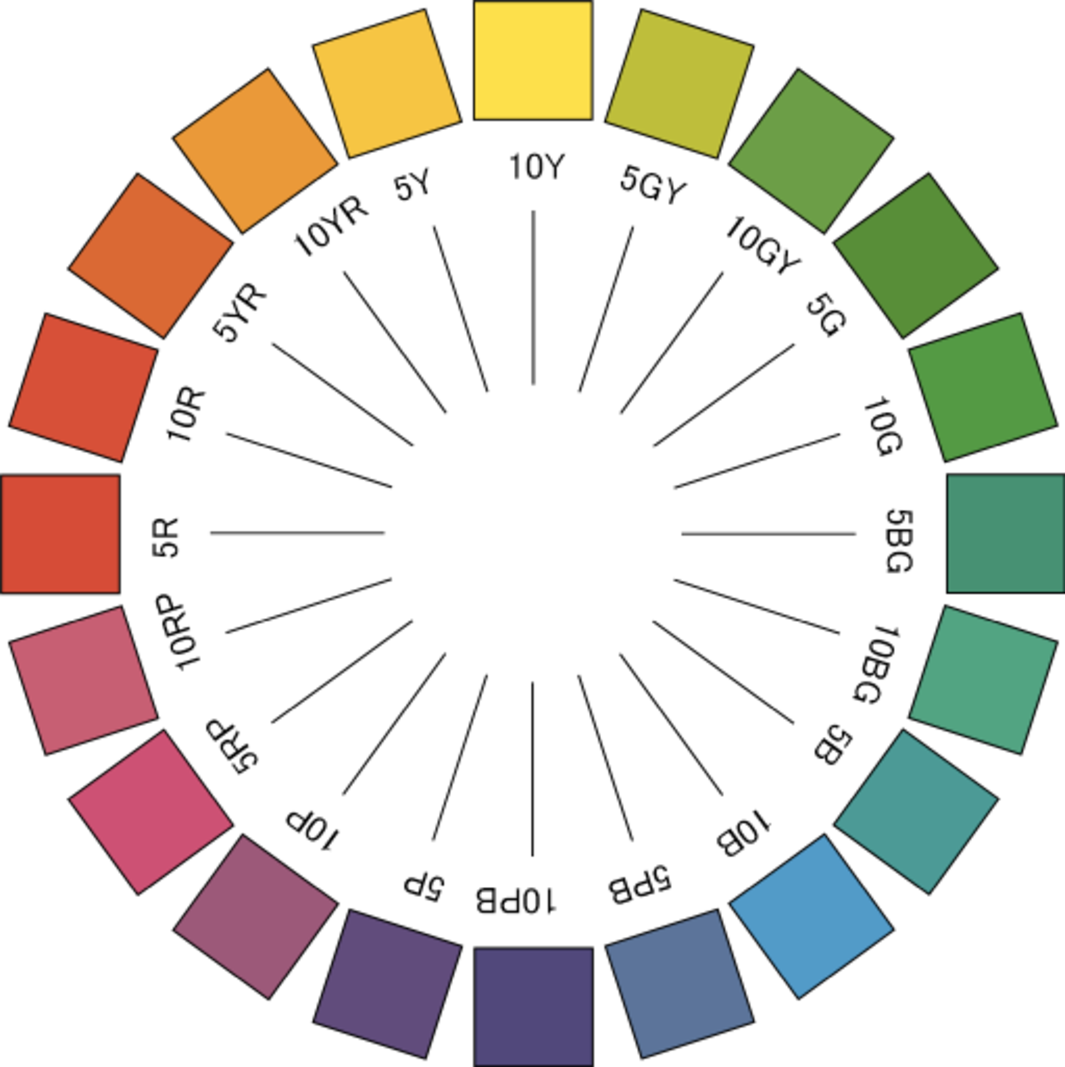
\includegraphics[height=5cm]{./spaces/figures/munsell-colour-wheel.pdf}
  \label{f:munsell-colour-wheel}
}
\subfigure[]{
  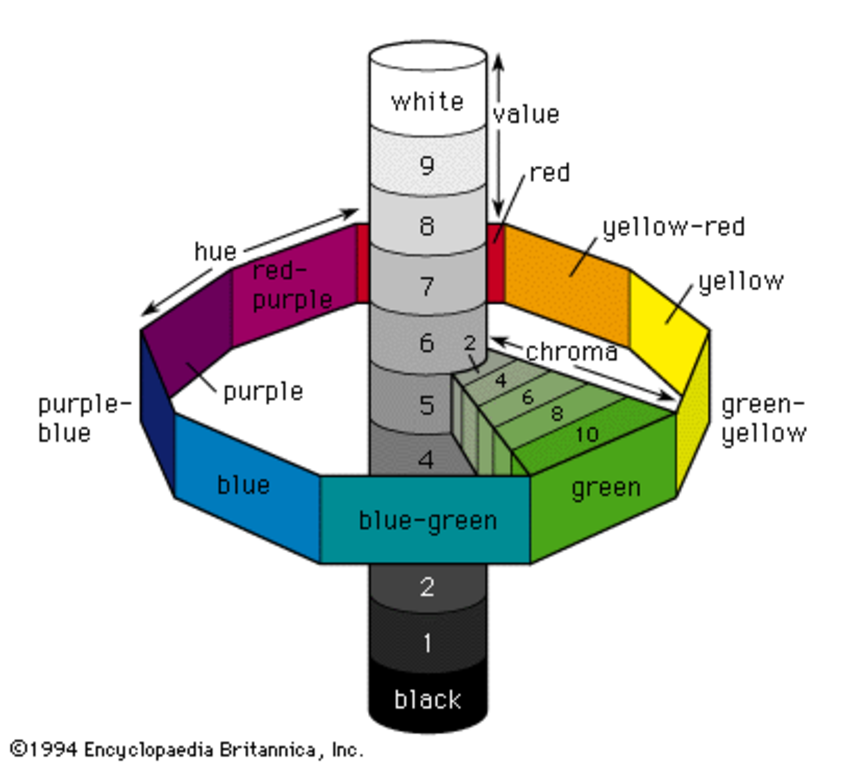
\includegraphics[height=5cm]{./spaces/figures/munsell-diagram-brittanica-1.pdf}
  \label{f:munsell-diagram}
}
\caption[The Munsell colour system]{\subref{f:munsell-colour-wheel}: a colour wheel representing different hue values in the Munsell colour system; \subref{f:munsell-diagram}: a diagram representing the three dimensions of the Munsell colour system: hue, value and chroma.}
\end{figure}

\subsection{Development}

The original goals of Albert H. Munsell were to develop a system that
is both psychophysically equidistant, meaning that it faithfully
represents the differences between different colours as experienced by
human subjects, and precisely applicable.

The development of the Munsell hue and chroma scales, which lead to
publication of the first Book of Color in 1929, is poorly documented
\citep{berns82development}. Only the research leading to the scale for
value has been properly documented but was based on the judgment of a
low number of human subjects (six to fourteen). A projection of the
colour samples in the Book of Color of 1929 on the \emph{a*b*} plane
of the CIE \emph{L*a*b*} colour space is shown in Figure
\ref{f:book-of-color-1929}.

\begin{figure}[htbp]
\begin{center}
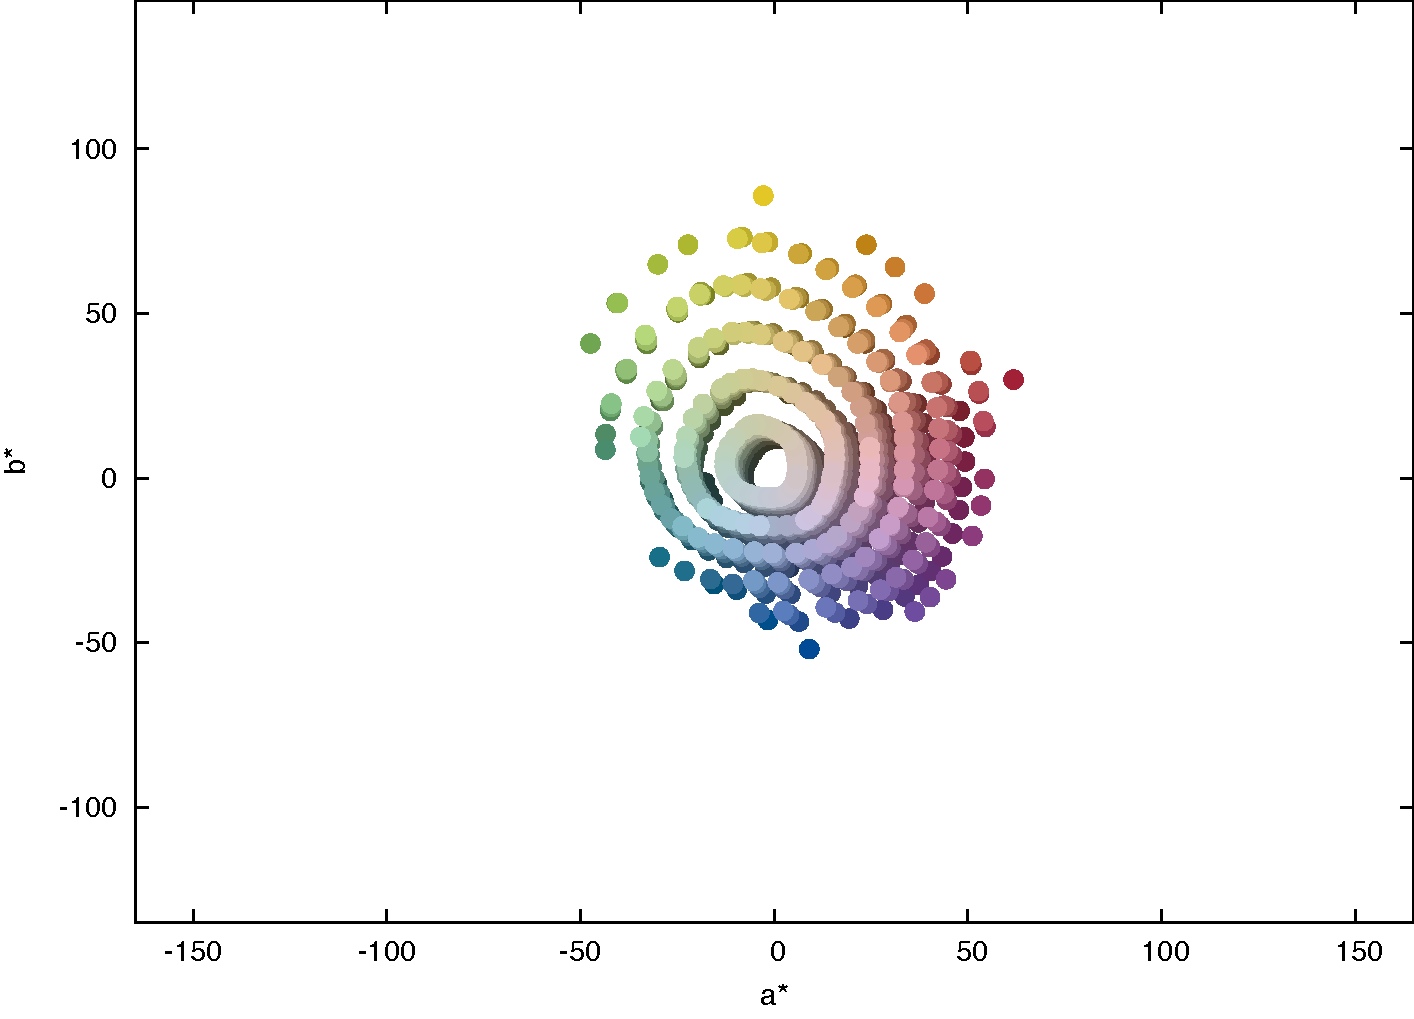
\includegraphics[width=.85\textwidth]{./spaces/figures/book-of-color-1929.pdf}
\caption[Colour samples of The Munsell Book of Color of 1929]{A projection of the colour samples that appear in the Munsell Book of Color of 1929 on the \emph{a*b*} plane of the CIE \emph{L*a*b*} colour space.}
\label{f:book-of-color-1929}
\end{center}
\end{figure}

Most of the shortcomings have been addressed in a follow-up study
\citep{newhall42final}, which critically reviewed and extensively
revised all three dimensions based on the judgment of fourty
participants and on more recent psychophysical findings. This study
also enlarged the Munsell solid to incorporate all colours within the
MacAdam limits, which is the theoretical maximum visual reflectance
factor for specified chromaticities \citep{macadam35maximum}. A
projection of the resulting colour samples on the \emph{a*b*} plane of
the CIE \emph{L*a*b*} colour space is shown in Figure
\ref{f:munsell}. These colour samples clearly cover a wider range of
possible colours when compared to those of the Book of Color in Figure
\ref{f:book-of-color-1929}.

\begin{figure}[htbp]
\begin{center}
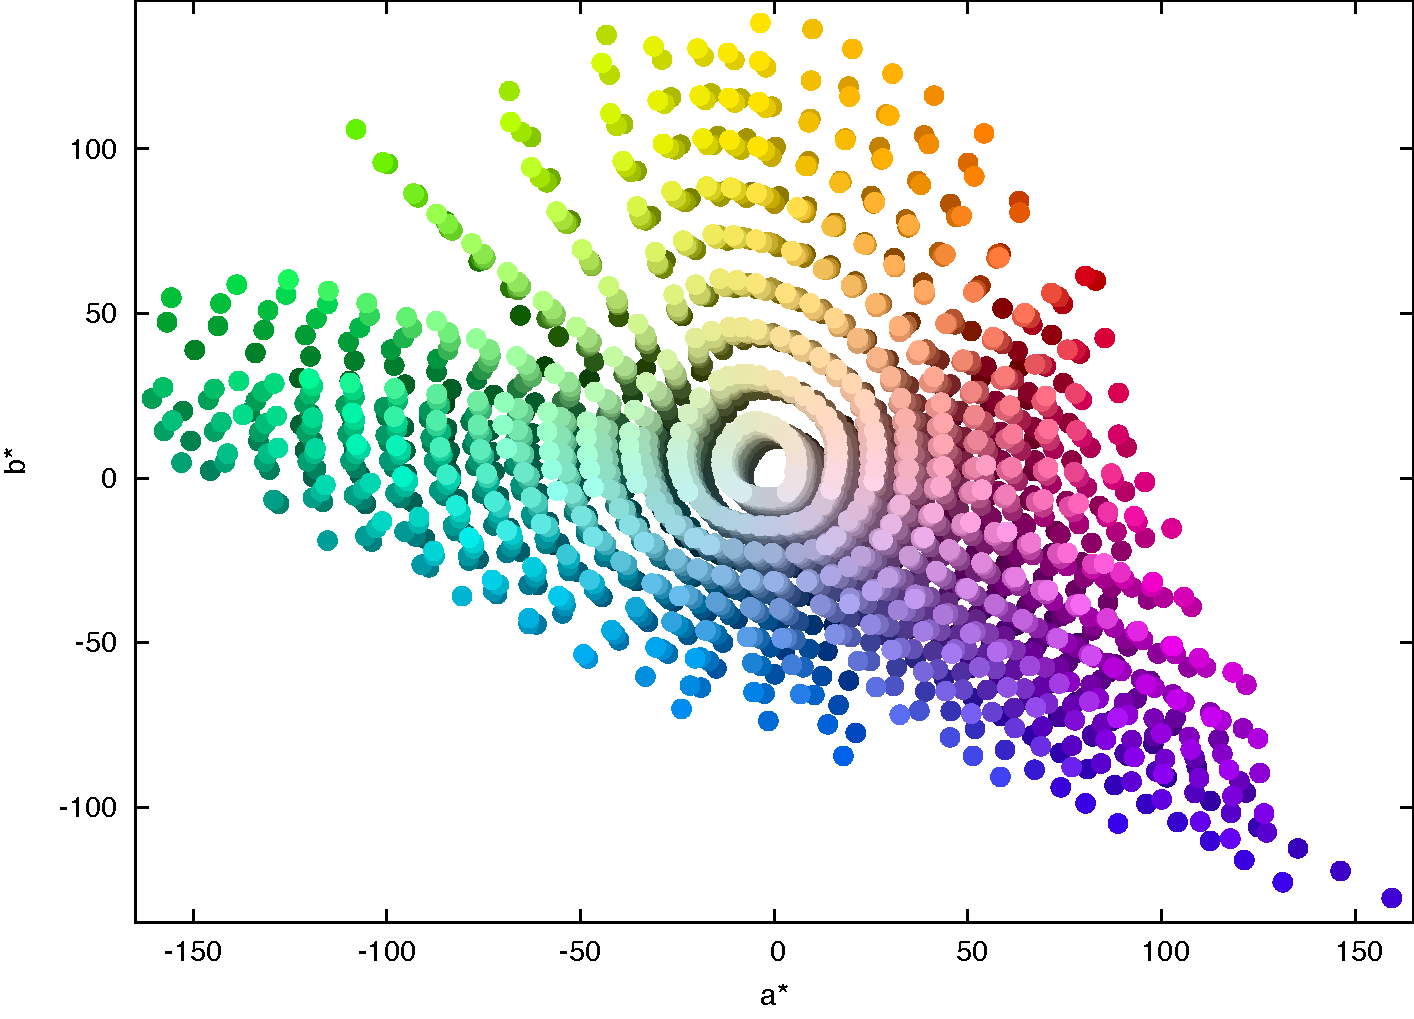
\includegraphics[width=.85\textwidth]{./spaces/figures/real.pdf}
\caption[Colour samples resulting from a study by
\citeauthor{newhall42final}]{A projection of the colour samples
  resulting from the study by \citeauthor{newhall42final} on the
  \emph{a*b*} plane of the CIE \emph{L*a*b*} colour space.}
\label{f:munsell}
\end{center}
\end{figure}

\subsection{Conversion}

The Munsell Color Science Laboratory, a research laboratory supported
by the Munsell Color Foundation at the Rochester Institute of
Technology, released three datafiles\footnote{Publicly available at
  \url{http://www.cis.rit.edu/mcsl/online/munsell.php}.} which map
colour chips from the Munsell colour system to corresponding CIE $xyY$
coordinates. One of these datafiles lists all Munsell colour chips
within the MacAdam limits as reported by \citet{newhall42final}. The
coordinates of most of these colours chips are only approximations
which are extrapolated or interpolated from a set of measurements of a
small subset of chips.

All coordinates stored in these datafiles use illuminant C. Care has
been taken to convert them to illuminant D65, using Equation
\ref{e:c-to-d65}, as this is the illuminant assumed in all experiments
reported in this book.

\section{Natural Color System}
\label{s:NCS}
\is{colour system!Natural}
\is{NCS|see{Natural Color System}}
\is{Natural Color System|see{colour system}}

The Natural Color System (NCS) is a proprietary colour system is based on 
Hering's opponent-colour theory. A colour is defined by three attributes:
\emph{blackness} (s), \emph{chromaticness} (c) and \emph{hue}
($\varphi$). A yellow colour for example can be described as 0580-Y10R,
where 05 corresponds to 5\% blackness, 80 to 80\% chromaticness and
Y10R to a hue of 90\% yellow and 10\% red.

Converting colours reported in the Natural Color System can be done
most precisely using a lookup table (SIS SS 19104), which describes
tristimulus values for NCS coordinates and can be obtained from national
standardization offices. \cite{derefeldt86transformation} report on an
approximative method to transform NCS coordinates to the CIE
$L^*a^*b^*$ colour space. In this book, I use the NCS navigator 
software\footnote{Available online at \url{http://www.ncscolour.com}.}
to compute the same conversion. This software is more precise 
than the method suggested by \cite{derefeldt86transformation}, but returns 
only integer values in the CIE $L^*a^*b^*$ colour space. Moreover, not all
colour samples are present in the software. Whenever a colour sample
was missing in the software, it was approximated using the nearest
colour sample that was available in the software.

\section{RGB}
\label{s:RGB}
\is{colour model!RGB}
\is{RGB|see{colour model}}

RGB is a technical colour model that is used in a wide range of
devices, such as in television sets and computer screens, to reproduce
colours. It is highly device-dependent as each RGB device comes with
its own colour profile and needs to be approached with considerable
care when used in colour research. Efforts have been made to define a
common colour profile that could be supported by any RGB device, but
these can at best be simulated on RGB devices that are commonly used
as they are not natively supported.

Another important aspect of the RGB colour model is the gamma
correction, which is used to counter the non-linearity between the
voltage applied to electrons and the resulting brightness on a
screen. This correction can be approximated by raising the values by a
power of gamma, which for most devices has a value of 2.2. Before RGB
values are transmitted to a screen, they can be gamma compressed by
raising to the power of the inverse of gamma.

On a final note, RGB devices are not capable of reproducing all
colours of the complete colour gamut, but of reproducing rather a
(small) subset of it. For example, both the Adobe RGB (1998) and
PAL/SECAM colour profile encode only half of the complete gamut. This
is the reason why some of the colour chips that are known to be foci
of basic colour categories, such as orange, can not be reproduced on
an everyday colour device.

The equations to convert any XYZ value using the D65 reference white,
to an RGB value for a device that is using the Adobe RGB (1998) colour
profile and a gamma correction of $\gamma$ is shown in Equations
\ref{e:xyz-rgb-first} and \ref{e:xyz-rgb-last}. When the values for
$R_t$, $G_t$ or $B_t$ are not within the range between 0 and 1, they
are not reproducable using this colour profile.

\begin{equation}
\begin{bmatrix}
  R_t \\ G_t \\ B_t
\end{bmatrix}
=
\begin{bmatrix}
 2.04148 & -0.0564977 & -0.344713 \\
-0.969258 & 1.87599& 0.0415557 \\
0.0134455  &  -0.118373 & 1.01527
\end{bmatrix}
\begin{bmatrix}
  X \\ Y \\ Z
\end{bmatrix}
\label{e:xyz-rgb-first}
\end{equation}

\begin{equation}
R = R_t^{1/\gamma} \quad G = G_t^{1/\gamma} \quad B = B_t^{1/\gamma}
\label{e:xyz-rgb-last}
\end{equation}

\section{YCbCr}
\label{s:ycbcr}
\is{colour model!YCbCr}
\is{YCbCr|see{colour model}}

Robotic vision data is typically delivered by one of the cameras in
the head or body of the robot. The colour information that is recorded
by these cameras can be stored in a wide variety of encodings. The
robots that have been used in my experiments deploy the YCbCr colour
model. In order to utilise this information, it needs to be converted
to the XYZ colour space, which happens in two steps. First it needs to
be converted to a RGB colour model using the Equations
\ref{e:ycbcr-rgb-first}-\ref{e:ycbcr-rgb-last}. Finally, these
coordinates can be converted to the XYZ using Equations
\ref{e:secam-rgb-xyz-first} and \ref{e:secam-rgb-xyz-last} which
assumes the SECAM/PAL colour profile.

\begin{align}
R& = (Y + 1.402 (C_r - 128) \label{e:ycbcr-rgb-first}) / 255 \\
G& = (Y - 0.34414 (C_b - 128) - 0.71414 (C_r - 128)) / 255 \\
B& = (Y + 1.772 (C_b - 128)) / 255\label{e:ycbcr-rgb-last}
\end{align}

\begin{equation}
R_t = R^\gamma \quad G_t = G^\gamma \quad B_t = B^\gamma
\label{e:secam-rgb-xyz-first}
\end{equation}

\begin{equation}
\begin{bmatrix}
  X \\ Y \\ Z
\end{bmatrix}
=
\begin{bmatrix}
 0.4306190 & 0.3415419 & 0.1783091 \\
 0.2220379 & 0.7066384 & 0.0713236 \\
 0.201853  &  0.1295504 & 0.9390944
\end{bmatrix}
\begin{bmatrix}
  R_t \\ G_t \\ B_t
\end{bmatrix}
\label{e:secam-rgb-xyz-last}
\end{equation}